\chapter{Umsetzung}
\label{ch:implementation}


%
% Section: Auswahl der Anwendungsanforderungen
%
\section{Auswahl der Anwendungsanforderungen}
\label{sec:implementation:selection}
In Tabelle \ref{tab:dlt_relevant} wurden alle \ac{DLT}-relevanten Anforderungen aufgezeigt und in der Implementierung dieser Arbeit umgesetzt. Anforderungen, die nicht umgesetzt werden konnten oder für die eine Alternativ-Lösung gefunden wurde, werden im Folgenden genannt:\\
Damit ein Smart-Contract rechtskonform agiert und um die Vertragslogik nach geltendem deutschen Recht korrekt abzubilden, bedarf es ausführlicher rechtlicher Beratung durch entsprechende Experten und Anwälte. Dieser zeitaufwändige Prozess wurde im Rahmen dieser Arbeit nicht berücksichtigt. Bei einer Implementierung, die über die Machbarkeitsstudie hinausgeht und produktiv eingesetzt werden soll, muss dieser Punkt berücksichtigt werden. Damit wurde Anforderung A1.3.2 nicht erfüllt.\\
Anforderung A1.2.5 beschreibt die Verschlüsselung von Transaktionsdaten, sodass Inhalte nur vom Eigentümer oder dem Adressaten einsehbar sind. Diese Funktionalität ist für das Zeigen der Machbarkeit einerseits nicht notwendig, für die Implementierung für ein Live-System jedoch essentiell. Gängige Methoden, um den Payload einer Transaktion zu verschlüsseln ist der Einsatz sogenannter Zero-Knowledge-Proofs (siehe \ref{XYZ}). Mit Hilfe dieses Ansatzes, ein Geheimnis zu beweisen ohne den Inhalt dabei preiszugeben, können in Kombination mit der Blockchain-Technologie Anwendungen entwickelt werden, die die Benutzerdaten vollständig schützen, ohne dabei an Funktionalität einzubüßen. Diese Anforderung wurde im Rahmen dieser Arbeit nicht umgesetzt.\\
Anforderung A1.3.8 beschreibt, dass Verträge im Nachhinein aktualisierbar sein müssen. Die Vertragslogik wurde mittels Smart-Contract umgesetzt: Einmal in der Blockchain gespeichert, sind Daten nicht mehr veränderlich. Es gibt dennoch Möglichkeiten, einen benötigten Mechanismus einzubauen, um die Verträge im Nachhinein anzupassen. Dazu kann man sich sogenannter Proxy-Smart-Contracts bedienen. Die Grundidee dabei ist, wie in einem Netzwerk ein zentrales Eingangstor zu haben, welches fest definiert ist und sich später nicht mehr ändert. Dieser Proxy verweist dann auf die jeweils aktuelle Version des benötigten Smart-Contracts. Ändert sich der Code durch Vertragsänderungen oder sonstige Updates, kann die aktualisierte Version in die Blockchain transferiert werden. Anschließend wird dem Proxy die Adresse des neuen Contracts mitgeteilt. Bei Anfragen an den Proxy leitet dieser den Anfragenden fortan an den neuen Vertrag weiter (der alte Vertrag bleibt dennoch weiterhin bestehen). Diese Umsetzung wurde im Zuge dieser Masterarbeit nicht geleistet, da die Umsetzung dieses Ansatzes viel Zeit und Aufwand benötigt, um die gewünschten Funktionalitäten zuverlässig zu implementieren. Da diese Arbeit als Machbarkeitsstudie aufgebaut wurde, wurde an dieser Stelle auf die Implementierung verzichtet. Es sei auf X und Y verwiesen; dort wird ein einfacher (allerdings nicht ausgereifter) Proxy-Smart-Contract vorgestellt. Die Nicht-Umsetzung dieser Anforderung verhindert nicht das Aufzeigen der generellen Machbarkeit.\\
Anforderung SA2.2.1 bezieht sich auf die Performanz, welche bei Ethereum mit etwa 20 Transaktionen pro Sekunde nicht ausreichend ist. Eine kurze Hochrechnung verdeutlicht die Problematik: Bei durchschnittlich drei Tassen Kaffee pro Mitarbeiter und Tag (9 Stunden von 08:00 Uhr bis 17:00 Uhr) und etwa 40 Mitarbeiter pro Kaffeemaschine (und Büro) ergibt sich bei 10.000 Maschinen eine benötigte Verarbeitungsgeschwindigkeit von 37 Tassen Kaffee pro Sekunde\footnote{Unter der Annahme, dass eine Tasse Kaffee mit einer Transaktion versendet wird.}. Damit wäre die Ethereum-Blockchain deutlich überlastet. Deshalb wurde sich hierbei einer alternativen Lösung bedient: Payment-Channel (vgl. Kapitel \ref{subsec:fundamentals:dlt:scaling}) werden eingesetzt, um das beschriebene Performanz-Problem zu lösen. Der Ansatz ist dabei wie folgt: Bei Vertragseröffnung wird gleichzeitig zwischen Kaffeemaschine und Benutzer ein Payment-Channel eröffnet. Dieser wird mit einem Betrag aufgeladen (Prepaid; 10€), sodass schon vor der ersten Benutzung der Maschine ein Betrag zur Verbuchung zur Verfügung steht. Möchte der Benutzer einen Kaffee von der Maschine erhalten, so erstellt diese eine Quittung und überträgt diese per \ac{NFC} an das Smartphone des Benutzers. Dieser kann anschließend mit seinem auf dem Smartphone befindlichen Private-Key die Quittung signieren und der Kaffeemaschine damit bestätigen, diesen Kauf durchgeführt zu haben. Die Kaffeemaschine bekommt anschließend die signierte Quittung per \ac{NFC} zurückgesendet und kann die Signatur überprüfen. Ist diese korrekt, wird der Kaffee ausgegeben. Dieser Vorgang passiert offchain und wird nicht per Transaktion an die Blockchain übermittelt. Dieser Vorgang kann nun so oft wiederholt werden, bis das Guthaben im Payment-Channel aufgebraucht ist. Ist dies der Fall, so muss der Benutzer zunächst sein Guthaben neu aufladen. Die Kaffeemaschine hält die zuletzt signierte Quittung so lange vor, bis ein definierter Zustand eintritt\footnote{Da eine Kaffeemaschine in der Regel nicht in der Nacht benutzt wird, könnte im Zeitraum zwischen 6 Uhr abends und 6 Uhr Morgens die Synchronisation stattfinden, sofern das Prepaid-Guthaben unter ein festgelegtes Minimum sinkt.}. Anschließend schickt sie diese Quittung per Transaktion an die Blockchain und erhält das entsprechend signierte Guthaben aus dem Payment-Channel. Dadurch kann die Zahl von etwa 1,2 Mio. Transaktionen pro Tag auf ein Bruchteil reduziert werden.

\subsection{Architektur und Aufbau}
\label{subsec:implementation:poc:architecture}


\begin{figure}[h]
 \centering
 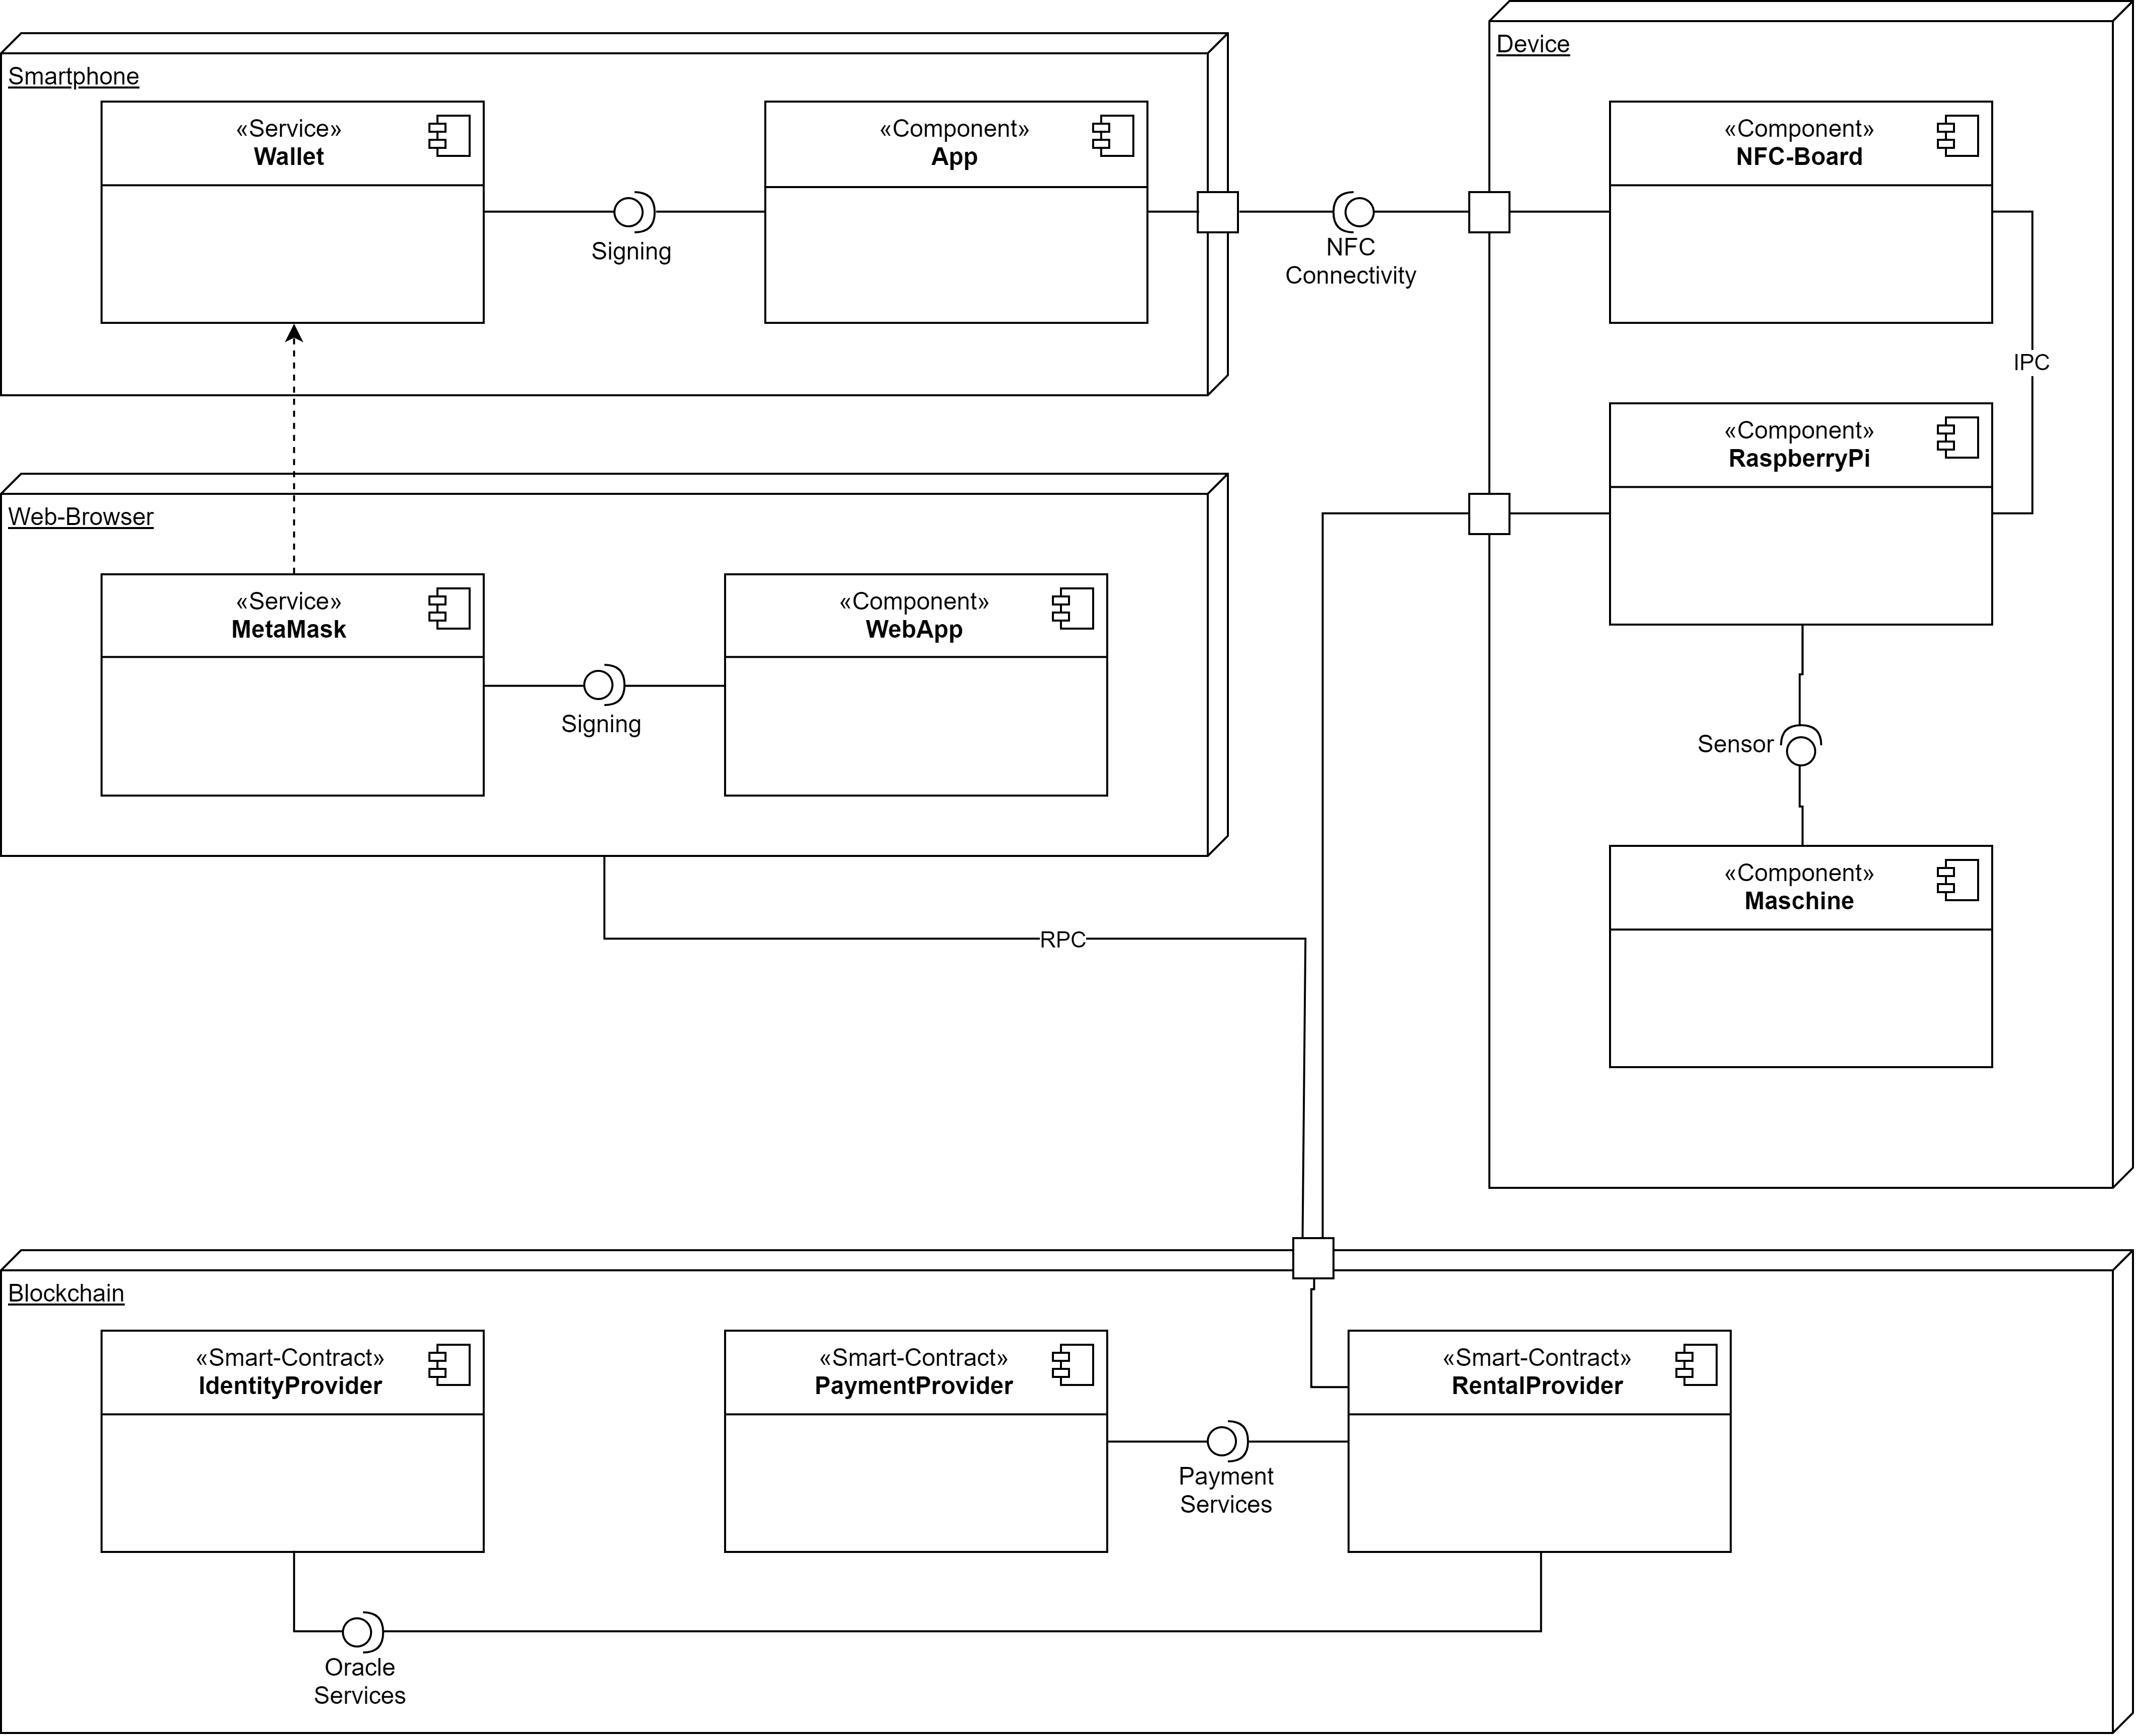
\includegraphics[width=1.0\textwidth]{gfx/Architecture.png}
 \caption{Architektur als UML-Komponentendiagramm}
 \label{fig:chapter07:architecture}
\end{figure}

Web-Applikation in React
Wallet als Browser-Plugin (Metamask)
Smart-Contracts für Mietverträge, Zahlungsabwicklung und Identitätsmanagement (Oracle) auf Kovan Testnet
Kaffeemaschine simuliert mittels Raspberry-Pi, angeschlossenes NFC-Entwicklungsboard
Smartphone als Wallet und zum Kommunizieren mit der Kaffeemaschine


\section{Testaufbau}
\label{subsec:implementation:poc:testing}
Die Vertragslogiken der Mietverträge wurden als Smart-Contracts in der Programmiersprache Solidity auf der Ethereum-Blockchain entwickelt. Für Smart-Contracts auf Ethereum-Basis existiert die Truffle-Suite, die ein umfangreiches Toolset für die Entwicklung und das Testen von Smart-Contracts bereitstellt. Mittels Unit-Tests wurde sichergestellt, dass die Funktionalität gemäß den Anforderungen gegeben ist.

Test-Coverage mit solidity-coverage

Hochrechnung Skalierungsansatz
Untersuchung Datenschutz und Privatsphäre
